\chapter{Generating surfaces}
\hl{Stuff to define?}
\begin{itemize}
    \item fBm surfaces
    \item Hurst exponent
    \item Gaussian random variable ?
    \item non-stationary
    \item self-similar
    \item isotropic
    \item lacunarity
\end{itemize}

Introduction?
% When generating random surfaces we want to be able to control the properties like the Hurst exponent (\hl{etc.?}) of the surface.

To generate our random surfaces we use an iterative midpoint displacement method usually called successive random additions \hl{(SRA)}. The method is based on a method proposed by Fourner in 1982\cite{fournier1982computer}, but with some modifications suggested by Voss\cite{voss1985random, voss1988fractals}. The method has further been discussed by Saupe\cite{saupe1988algorithms}, amongst others. We choose this method mainly because it's possible to generate periodic surfaces with it, because it generates very good approximations to fBm surfaces\cite{zhou2005comparison}, and because the Hurst exponent of the generated surfaces is easy to control. The method is also easy to understand, easy to implement, and generates surfaces with high resolution very fast. The method is widely used in scientific applications\hl{cite??} because of these properties, and is also used for generating surfaces in computer graphics, since the surfaces look very realistic \hl{with only some minor artefacts?? (high, narrow peaks)}.

\section{Midpoint displacement methods (in 1 dimension)}
\todo[inline]{The most basic method we used is a very basic but widely used method, which has many variations and names. The most common names are ``the diamond-square algorithm''\hl{cite}, ``the midpoint displacement method''\hl{cite}, ``plasma fractal'' and ``cloud fractal''.}

The method we use to generate random surfaces is very similar to the standard midpoint displacement method, which in 1 dimension goes as follows. See \cref{fig:midpoint01} for a visual presentation.
%
\begin{enumerate}
    \item Give the values at the endpoints of the interval, $y_0$ and $y_n$, random values from a Gaussian random variable with mean $\mu = 0$ and variance $\sigma_0^2$. This initial standard deviation $\sigma_0$ can be chosen freely.
    \item Generate the value in the center of the interval, $y_{n/2}$, by averaging over the two endpoints and adding a Gaussian random number with mean $\mu = 0$ and a \emph{reduced} variance
    \begin{align}
         \sigma_1^2 = \left(1/2\right)^{2H}\sigma_0^2, \label{eq:midpoint_sigma_first}
    \end{align}
    where $H$ is the wanted Hurst exponent.
    \item Continue generating the values in the center of each sub-interval until you reach the desired number of points, while reducing the variance of the random number by a factor $\frac{1}{2}$ each iteration\todo{Why 1/2? (needed to create good approx. to fBm, see \cite{voss1985random})}. For iteration $i$ we have
    \begin{align}
        \sigma_i^2 = \left(1/2\right)^{i2H}\sigma_0^2. \label{eq:midpoint_sigma_general}
    \end{align}
\end{enumerate}
%
\begin{figure}[htpb]%
    \centering%
    \includesvg[width=0.5\textwidth, svgpath=./images/diamond_square/]{random_midpoint_displacement_regular02}%
    \caption{%
        \hl{Illustration of the midpoint displacement method in 1 dimension. We increase the number of points from 2 to 9 using 3 iterations.}%
        \label{fig:midpoint01}%
    }%
\end{figure}%

This method generates a \hl{1-dimensional line}, with a Hurst exponent \hl{close} to the input $H$\todo{how close?}. But since we only add random numbers to the new values, the result is non-stationary for $H \neq 0.5$\cite{voss1985random}\hl{, and it is neither self-similar or isotropic, as noted by Mandelbrot}\cite{mandelbrot1982comment}. To mitigate this we implement the addition suggested by Voss\cite{voss1985random}, which consists of adding a random number to \emph{all} points in each iteration, both the new and old. Voss called this modified method \emph{successive random additions}.

\section{Successive random additions in 2 dimensions}
As mentioned \st{before}, the method called \emph{successive random additions} is a modification of the regular midpoint displacement method first described by Richard F. Voss\cite{voss1985random}, where we add random numbers to \emph{all} points in each iteration, compared to just the \emph{new} points in the regular midpoint displacement method. This modification means that we can replace the factor $(1/2)$ in \cref{eq:midpoint_sigma_first,eq:midpoint_sigma_general} with a general factor $r$\todo{why? (something about distance between points)}, and we get
\begin{align*}
    \sigma_i^2 = r^{2H}\sigma^2_{i-1}.
\end{align*}
\hl{$r$ controls the lacunarity/roughness, $H$ independent of $r$}

% \subsection{(on an infinite grid) in 2 dimensions}
\subsection{On an infinite grid}
Voss has geneneralized the the method of successive random additions to higher dimensions\cite{voss1985random}, and this generalized form is the algorithm we use when generating fractures. We generate surfaces in the form of heightmaps, meaning a 2-dimensional grid of points ({$x,y$}), with a value for the height in each point \hl{($z(x,y) = z_{x,y}$)} which is generated by the algorithm.

The central part of the algorithm consists of two steps often called the \emph{diamond-step} and the \emph{square-step}. We start with a simple case of an infinite grid of evenly spaced points, all with known $z$-values. The two steps are as follows:
\begin{description}
    \item[The \emph{square-step}:] The grid can be divided into small squares consisting of four points in each square, as in the leftmost square in \cref{fig:simple_square_step}. We generate the $z$-value in the center of each of these squares by averaging the $z$-values of the four corners of each square, as indicated by the red dots and arrows in \cref{fig:simple_square_step}. Then add a random Gaussian number with mean $\mu = 0$ and variance $\sigma_i^2 = \sigma_{i-1}^2r^{2H}$ to all new and old points, where $\sigma_{i-1}^2$ is the variance used in the last step of the algorithm.
    \label{enum:test}
    
    \item[The \emph{diamond-step}:] After the square-step the grid can be divided into smaller squares that are tilded by 45 degrees, as in the leftmost square in \cref{fig:simple_diamond_step}. We generate the $z$-values in the center of each square by averaging the $z$-values of the four corners of each square, as indicated by the red dots and arrows in \cref{fig:simple_diamond_step}. We then add a random Gaussian number with mean $\mu = 0$ and variance $\sigma_{i+1}^2 = \sigma_i^2r^{2H}$, to all new and old points. 
\end{description}
See \cref{fig:diamond_square_applied} for an illustration of the algorithm applied once on a larger grid. 

\begin{figure}[htpb]%
\centering%
%
\setlength{\myfigwidth}{0.5\textwidth}%
\setlength{\mycaptionwidth}{0.3\textwidth}%
%
% \parbox[c][2cm][c]{\myfigwidth}{
%     \includesvg[width=\myfigwidth, svgpath = images/diamond_square/]{simple_square_step_solarized08}
% }
% \parbox[c][2cm][c]{\mycaptionwidth}{
%     \subcaption{Square-step}
%     \label{fig:simple_square_step}
% }
%
% \begin{minipage}[c][2cm][c]{\myfigwidth}
%     \includesvg[height=2cm, svgpath = images/diamond_square/]{simple_square_step_solarized08}
% \end{minipage}
% \begin{minipage}[c][2cm][c]{\mycaptionwidth}
%     \subcaption{Square-step}
%     \label{fig:simple_square_step}
% \end{minipage}
%
\begin{minipage}[c]{\myfigwidth}%
    \includesvg[width=\textwidth, svgpath = images/diamond_square/]{simple_square_step_solarized08}%
\end{minipage}%
\begin{minipage}[c]{\mycaptionwidth}%
    \subcaption{Square-step}%
    \label{fig:simple_square_step}%
\end{minipage}%
\\%
\vspace{2mm}%
\begin{minipage}[c]{\myfigwidth}%
    \includesvg[width=\textwidth, svgpath = images/diamond_square/]{simple_diamond_step_solarized05}%
\end{minipage}%
\begin{minipage}[c]{\mycaptionwidth}%
    \subcaption{Diamond-step}%
    \label{fig:simple_diamond_step}%
\end{minipage}%
%
\caption{Illustration of the two steps used in the diamond square algorithm for generating random surfaces. The grey points are old points, the black points are new points, and the red points are the points used in the calcuation of the averages when generating the new points.}%
\label{fig:diamond_square_steps}%
\end{figure}%

We see that by first applying the square-step and then applying the diamond-step, we add one point in between each point in each direction, almost doubling the resolution of the grid. In general we go from $n$ to $n + (n-1)$ points in each direction. By applying the algorithm several times we get \todo{replace $n$ with $N$ and $i$ with $n$?}
\begin{align}
    n_1 &= n_0 + (n_0-1) = 2n - 1 \nonumber\\
    n_2 &= 2n_1 - 1 = 4n_0 - 3 \nonumber\\
    n_3 &= 2n_2 - 1 = 9n_0 - 7 \nonumber\\
    &\vdotswithin{=} \nonumber\\
%     &\shortvdotswithin{=}
    n_i &= 2^i(n_0-1) + 1, \label{eq:diamond_step_resolution}
\end{align}
where $i$ is the number of times we have applied the algorithm. This means that using the diamond-square algorithm we can go from any resolution $n_0$ to all resolutions satisfying $n_i = 2^i(n_0 - 1) + 1$.
%
\begin{figure}[htpb]%
    \centering%
    \includesvg[width=0.7\textwidth, svgpath = images/diamond_square/]{increase_resolution_solarized_starssquares03}%
    \caption{%
        The diamond-square algorithm applied once on a grid of $3\times 3$ points, increasing the number of points from 9 to 25. The orange square points are generated by the square-step (see \cref{fig:simple_square_step}), and the blue star-shaped points by the diamond-step (see \cref{fig:simple_diamond_step}).%
    }%
    \label{fig:diamond_square_applied}%
\end{figure}%

% \subsection{Successive random additions on a finite grid (in 2 dimensions)}
\subsection{On a finite grid}
Since we are using computers to generate our surfaces, which have limited memory, we can't use infinite grids. This means we get some special cases that needs to be taken care of when generating points near the edges of the grid.\todo{transition to below}

For the square step we generate one new point in the center each square formed by the grid from the previous iteration, and in general we generate the $z$-values in the points
\begin{align}
    &\left(x_{i+1/2}, y_{j+1/2}\right) &0\leq i,j < n, \label{eq:square_step_limits}
\end{align}
where $(x_i,x_j)$ are the points in the grid after the last iteration. In general the averages we calculate for the new points can be written as\todo{make this equation nicer}
% \begin{align}
%     (x_{i+1/2}, y_{j+1/2}) 
%     &= \frac{1}{4}\big(
%         (x_i, y_j) + (x_{i+1}, y_j)\nonumber\\
%         &+ (x_i, y_{j+1}) + (x_{i+1}, y_{j+1})
%     \big)
%     &0\leq i,j < n.
%     \label{eq:square_step}
% \end{align}
\begin{align}
    (x_{i+1/2}, y_{j+1/2}) 
    = \frac{1}{4}\big[
        (x_i, y_j) + (x_{i+1}, y_j)
        &+ (x_i, y_{j+1}) + (x_{i+1}, y_{j+1})
    \big],
    \label{eq:square_step}
\end{align}
using the limits in \cref{eq:square_step_limits}. We see that the square-step only uses points inside the grid, which means that we don't have to modify it when going to a finite grid.

For the diamond-step we generate the values in the points

\begin{align}
    &(x_{i+1/2}, y_j) &\text{for } 0\leq i<n \text{ and } 0\leq j \leq n& \label{eq:diamond_step_limits01}\\
    &(x_i, y_{j+1/2}) &\text{for } 0\leq i\leq n \text{ and } 0\leq j < n&. \label{eq:diamond_step_limits02}
\end{align}
In general the averages we calculate for the new points can be written as\todo{make these equations nicer}
% \begin{align}
%     (x_{i+1/2}, y_j) 
%     &= 
%     \frac{1}{4}\big(
%         (x_i, y_j) + (x_{i+1}, y_j) + (x_{i+1/2}, y_{j-1/2}) + (x_{i+1/2}, y_{j+1/2})
%     \big) \label{eq:diamond_step01}\\
%     (x_i, y_{j+1/2}) 
%     &= 
%     \frac{1}{4}\big(
%         (x_i, y_j) + (x_i, y_{j+1}) + (x_{i-1/2}, y_{j+1/2}) + (x_{i+1/2}, y_{j+1/2})
%     \big). \label{eq:diamond_step02}
% \end{align}
\begin{align}
    (x_{i+1/2}, y_j) 
    &= 
    \frac{1}{4}\big[
        (x_i, y_j) + (x_{i+1}, y_j) \nonumber\\
        &+ (x_{i+1/2}, y_{j-1/2}) + (x_{i+1/2}, y_{j+1/2})
    \big]
    \label{eq:diamond_step01}\\
    (x_i, y_{j+1/2}) 
    &= 
    \frac{1}{4}\big[
        (x_i, y_j) + (x_i, y_{j+1}) \nonumber\\
        &+ (x_{i-1/2}, y_{j+1/2}) + (x_{i+1/2}, y_{j+1/2})
    \big],
    \label{eq:diamond_step02}
\end{align}
using the limits in \cref{eq:diamond_step_limits01,eq:diamond_step_limits02}. We now see that when generating points near the edges using the diamond-step, specifically when generating the points $(x_{i+1/2}, y_j)$ for $j \in \{0, n\}$ and $(x_i, y_{j+1/2})$ for $i = \{0, n\}$, we need to average over points that lie outside the grid. There are two possible solutions, depending on the surface we are generating. If generating a periodic surface, the solution is to wrap around the edges using periodic boundary conditions, and find the point we need on the opposite side of the grid. For example (using $i = j = 0$)
\begin{align*}
    (x_{1/2}, y_{-1/2}) = (x_{1/2}, y_{n-1/2}).
\end{align*}
If generating a non-periodic grid we simply ignore the points that lie outside the grid when calculating the averages, and just use the \hl{three/3} other points.

% \subsection{Implementing successive random additions (on a finite grid in 2 dimensions)}
\subsection{Implementation}
In our implementation we generate a surface on a finite grid of size $N\times N$, starting with only the $z$-values in the four corners defined, giving a resolution $n_0 = 2$. As shown in \cref{eq:diamond_step_resolution} the algorithm can go from any resolution $n_0$ to any resolution \hl{of the form} $n_p = 2^p(n_0-1) + 1$ by applying the algorithm $p$ times, which means that our implementation can generate surfaces with resolutions
\begin{align*}
    N &= 2^p(2-1) + 1 = 2^p + 1,
\end{align*}
where $p$ is any positive integer.

We implement generation of both periodic and non-periodic surfaces using using \crefrange{eq:square_step_limits}{eq:diamond_step02}, while skipping points outside the grid for non-periodic surfaces, and wrapping around the edges using periodic boundary conditions when generating periodic surfaces.

To ensure that the periodic surfaces actually turn out periodic we start with all four corners having the same value. We also let the right and bottom edge be equivalent to the left and top edge, respectively, which effectively means that all four corners should always have the same $z$-value. To ensure that the opposite edges stay equal to each other we never generate any points on the right and bottom edge, but just copy the $z$-values from the opposite \hl{corresponding} edge after the diamond-step.

This leaves us with the following algorithm for generating a surface which approximates a 2-dimensional fractional Brownian motion with Hurst exponent $H$
\begin{enumerate}
    % \itemsep1pt \parskip0pt \parsep0pt
    \renewcommand{\labelitemii}{$\bullet$}
    
    \item Allocate a grid of size $N\times N$, where $N = 2^p + 1$, and $p$ is any positive integer. \hl{This grid will store the $z$-values, or the height of the surface, in each grid point $(x,y)$.}

    \item Initialize the $z$-values of the corners of the grid by drawing random numbers from a Gaussian distribution with mean $\mu = 0$ and variance $\sigma_0$. The initial variance can be chosen freely. \hl{The initial resolution is now $n_0\times n_0$, with $n = 2$}.
    \begin{itemize}
        \item If generating a periodic surface, give all four corners the same $z$-value.
    \end{itemize}
    
    \item Apply the square-step using \cref{eq:square_step_limits,eq:square_step}. Add a random Gaussian number with mean $\mu = 0$ and variance $\sigma_i = \sigma_{i-1}^2r^{2H}$ to all new and old points.
    \label{enum:square_step}

    \item Apply the diamond-step using \crefrange{eq:diamond_step01}{eq:diamond_step02}. Add a random Gaussian number with mean $\mu = 0$ and variance $\sigma_{i+1} = \sigma_i^2r^{2H}$ to all new and old points.
    \label{enum:diamond_step}
    
    \begin{itemize}
        \item If generating a periodic surface, skip generating $z$-values for points on the right and bottom edge using the diamond-step, and instead copy the values from the opposite edges after the diamond-step.
    \end{itemize}
    
    \item Repeat step \ref{enum:square_step} and \ref{enum:diamond_step} $p$ times until you reach the desired resolution of $N\times N$, where $N = 2^p + 1$. For step $i$ the variance of the random Gaussian numbers is
    \begin{align*}
        \sigma_i^2 = \sigma_0^2(r^i)^{2H}.
    \end{align*}
\end{enumerate}

See \cref{fig:diamond_square_surface} for a surface generated by the algorithm.
%
% \begin{figure}[htpb]%
%     \centering%
%     \includesvg[width=0.7\textwidth, svgpath=./images/diamond_square/surface_example/]{surface_labels}%
%     \caption{%
%         Caption.%
%         \label{fig:diamond_square_surface}%
%     }%
% \end{figure}%
\begin{figure}[htpb]%
    \centering%
    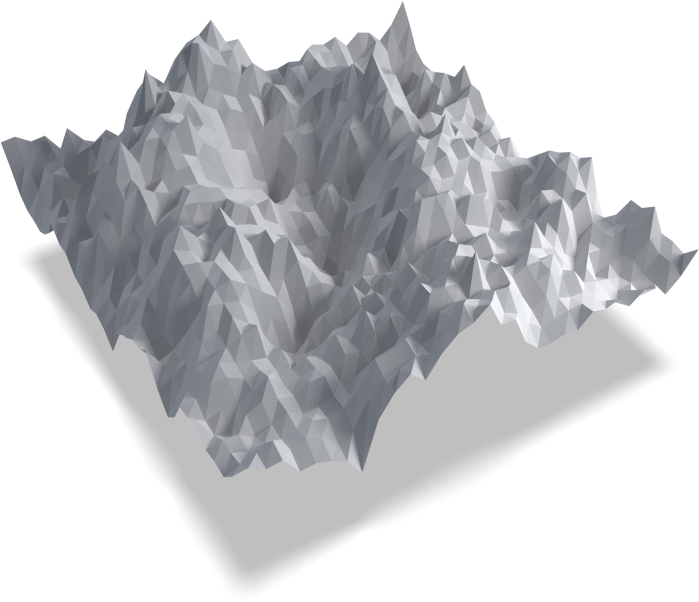
\includegraphics[width=0.5\textwidth]{./images/diamond_square/surface_blender/surface_composite01_cropped.png}%
    \caption{%
        Caption.%
        \label{fig:diamond_square_surface}%
    }%
\end{figure}%

\orangebox{
{\bf Notes:}
\begin{itemize}
    \item Implementation (in Matlab/C++)?
    \item periodic and non-periodic
    \item Mention that DS can be used to increase resolution of any surface
    \item Can increase resolution of generated surface, if we know the seed
\end{itemize}

{\bf Stuff to define:}
\begin{itemize}
    \item Periodic/non-periodic
    \item Lacunarity
\end{itemize}
}

\subsection{Testing the method}
%
\begin{figure}[htpb]%
    \centering%
    {
        \newcommand{\f}{\footnotesize}%
        \newcommand{\x}{\text}%
        \newcommand{\hh}{{\f $H_\x{in}=H_\x{out}$}}%
        \includesvg[width=0.7\textwidth, svgpath=./images/diamond_square_Hurst/test_diamondSquare/]{fig01}%
    }
    \caption{%
        Diamond square accuracy? Measured using DMA. The dashed grey line indicates a measured Hurst exponent of 0.75, the solid grey line a measured exponent exactly equal to the input exponent. The green lines are surfaces created using periodic boundary conditions (PBC), the red lines using non-periodic boundaries, the dashed lines using successive random additions (SRA), and the solid lines using the regular midpoint displacement method (MDM). \hl{FINISH CAPTION}. %
%         \label{fig:cell_lists}%
    }%
\end{figure}%
